\documentclass[twocolumn]{article}

% Standard packages for Bioinformatics template approximation
\usepackage{graphicx}
\usepackage{amsmath}
\usepackage{booktabs}
\usepackage{hyperref}
\usepackage{geometry}
\usepackage{caption}

% Approximate journal margins and 86mm columns
\geometry{a4paper, margin=1.5cm, columnsep=0.8cm}

\title{Identification of Fibromyalgia Biomarkers through Gene Expression Dimensionality Reduction and Logistic Regression}

\author{
    Giovanni Russo Paschoal \\
    \small \textsuperscript{1}Department of Computer Science, Universidade Federal de Minas Gerais (UFMG),\\
    \small Belo Horizonte, MG, 31270-901, Brazil
}
\date{}

\begin{document}

\maketitle

\section*{Abstract}
\textbf{Motivation:} Fibromyalgia (FMA) is a chronic pain syndrome with an elusive etiology. It currently lacks observable biomarkers in the bloodstream through common methods, making it a diagnosis of exclusion based on clinical symptoms. Identifying predictive genomic markers is crucial for robust diagnostic procedures. \\
\textbf{Results:} Using high-throughput RNA sequencing data (GSE221921) from 189 subjects (96 FMA patients and 93 healthy controls), we structured a Vector Space Model (VSM) to classify patients based on 21,446 expressed genes. By solving an augmented sparse linear system, we extracted initial regression weights, isolating the 42 most relevant markers. To prevent sex-based variance bias, we filtered out chromosome X and Y genes via the \textit{mygene.info} API, yielding a refined subset of 33 non-sexual genes. Applying Truncated Singular Value Decomposition (SVD), we demonstrated that the reduced dataset features 2 to 3 dominating singular values, clearly separating the classes in a 3D principal component space while drastically reducing noise. A Logistic Regression classifier trained on the SVD components achieved robust accuracy in distinguishing FMA patients from the control group, both on an independent holdout test set and under Stratified 5-Fold Cross-Validation.\\
\textbf{Availability and Implementation:} The initial dataset is available at NCBI GEO (accession GSE221921). The MATLAB and Python implementation scripts for filtering, SVD, and classification are freely available at \url{https://github.com/GiorussoP/bioinformatics.git}.\\
\textbf{Contact:} \href{mailto:giovanni@ufmg.br}{giovanni@ufmg.br} \\
\textbf{Supplementary information:} An animated rotation of the 3D SVD scatter plot (Figure~\ref{fig:svd_3d}) is provided as a supplementary GIF file; additional supplementary data are available at \textit{Bioinformatics} online.

\section{Introduction}
Fibromyalgia (FMA) is a chronic syndrome characterized by widespread musculoskeletal pain, fatigue, and cognitive difficulties. The major clinical challenge lies in the absence of validated physiological biomarkers, forcing clinicians to rely on exclusionary diagnostic criteria.

Recent advancements in High-throughput RNA sequencing (RNA-Seq) allow for the quantification of dysregulated genes in FMA patients. By translating these expression profiles into a machine learning context, we can construct a Vector Space Model (VSM) where patients act as independent entities and transcribed genes act as continuous dimensions. The objective of this study is to group these coordinates, segregating vectors of FMA patients from healthy ones to discover actionable biological markers.

\section{System and methods}

\subsection{Data Preparation and Microarray Adaptation}
We utilized the GSE221921 dataset comprising 189 samples (96 FMA cases, 93 matched controls). The raw matrix originally contained 21,915 targets. To adapt the asymmetrical RNA-Seq output (FPKM) to a standard Microarray analysis, we discarded spatial metrics (Start, End, Karyotype) and applied a logarithmic compression defined by $\log_2(\text{value} + 1)$. Missing values were handled by discarding genes with omitted canonical symbols ($\sim2.14\%$), leaving 21,446 valid dimensions. Calibration elements (e.g., \texttt{AFFX-}, \texttt{ERCC-}) were also removed.

\subsection{Feature Selection via Logistic Regression}
To identify initial biomarker candidates, we solved a linear regression system using the complete scaled matrix $A$ and a class target vector $b$. A sparse matrix formulation $M$ was constructed to calculate the weights $w$:
\begin{equation}
M = \begin{bmatrix} I_m & -A \\ A' & I_n \end{bmatrix}, \quad M x = n_b
\end{equation}
where $n_b$ is a zero vector augmented with $-b$. The resulting magnitudes $|w|$ were sorted descendingly to extract a reduced matrix $A_r$ composed of the $n_{attr} = 42$ most discriminative attributes.

\subsection{Chromosomal Filtering}
Since variance in gene expression can be skewed by sexual dimorphism, we systematically removed genes located on the X and Y chromosomes. A Python pipeline queried the HGNC symbols against the \textit{mygene.info} API, verifying the \texttt{genomic\_pos.chr} parameter. This process isolated 33 core non-sexual genes (e.g., PCSK5, FAM160A1).

\subsection{Dimensionality Reduction (SVD)}
We applied Truncated Singular Value Decomposition (SVD) on both the full ($A$) and reduced ($A_r$) matrices. SVD factorizes the matrix such that $A_r = U \Sigma V^T$. The diagonal elements of $\Sigma$ (singular values) were plotted to evaluate the significance of directional variance.

\subsection{Classification}
Using the refined 33-gene matrix, we employed a pipeline integrating \texttt{StandardScaler}, \texttt{TruncatedSVD} ($n=5$), and \texttt{LogisticRegression} with balanced class weights. To assess generalization to previously unseen samples, the 189 patients were first split into a training set (70\%) and an independent holdout test set (30\%) using stratified sampling, preserving the FMA/Healthy class proportions in both partitions. All preprocessing steps (scaling and SVD) were fitted exclusively on the training partition and subsequently applied to the holdout set, which was used only once for final evaluation. As a complementary robustness check, the full pipeline was additionally evaluated on the entire dataset via Stratified 5-Fold Cross-Validation.

\section{Results}

\subsection{Attribute Selection}
The initial linear prediction over the full matrix $A$ contained significant noise. However, extracting the 42 attributes with the highest magnitudes yielded a significantly cleaner probability distribution. Figure \ref{fig:reg_log} illustrates the logistic progression curve and the separation obtained by varying the number of selected attributes.

\begin{figure}[h]
    \centering
    % Placeholder for reg_log.m outputs (Plot 1, Plot 2, etc.)
    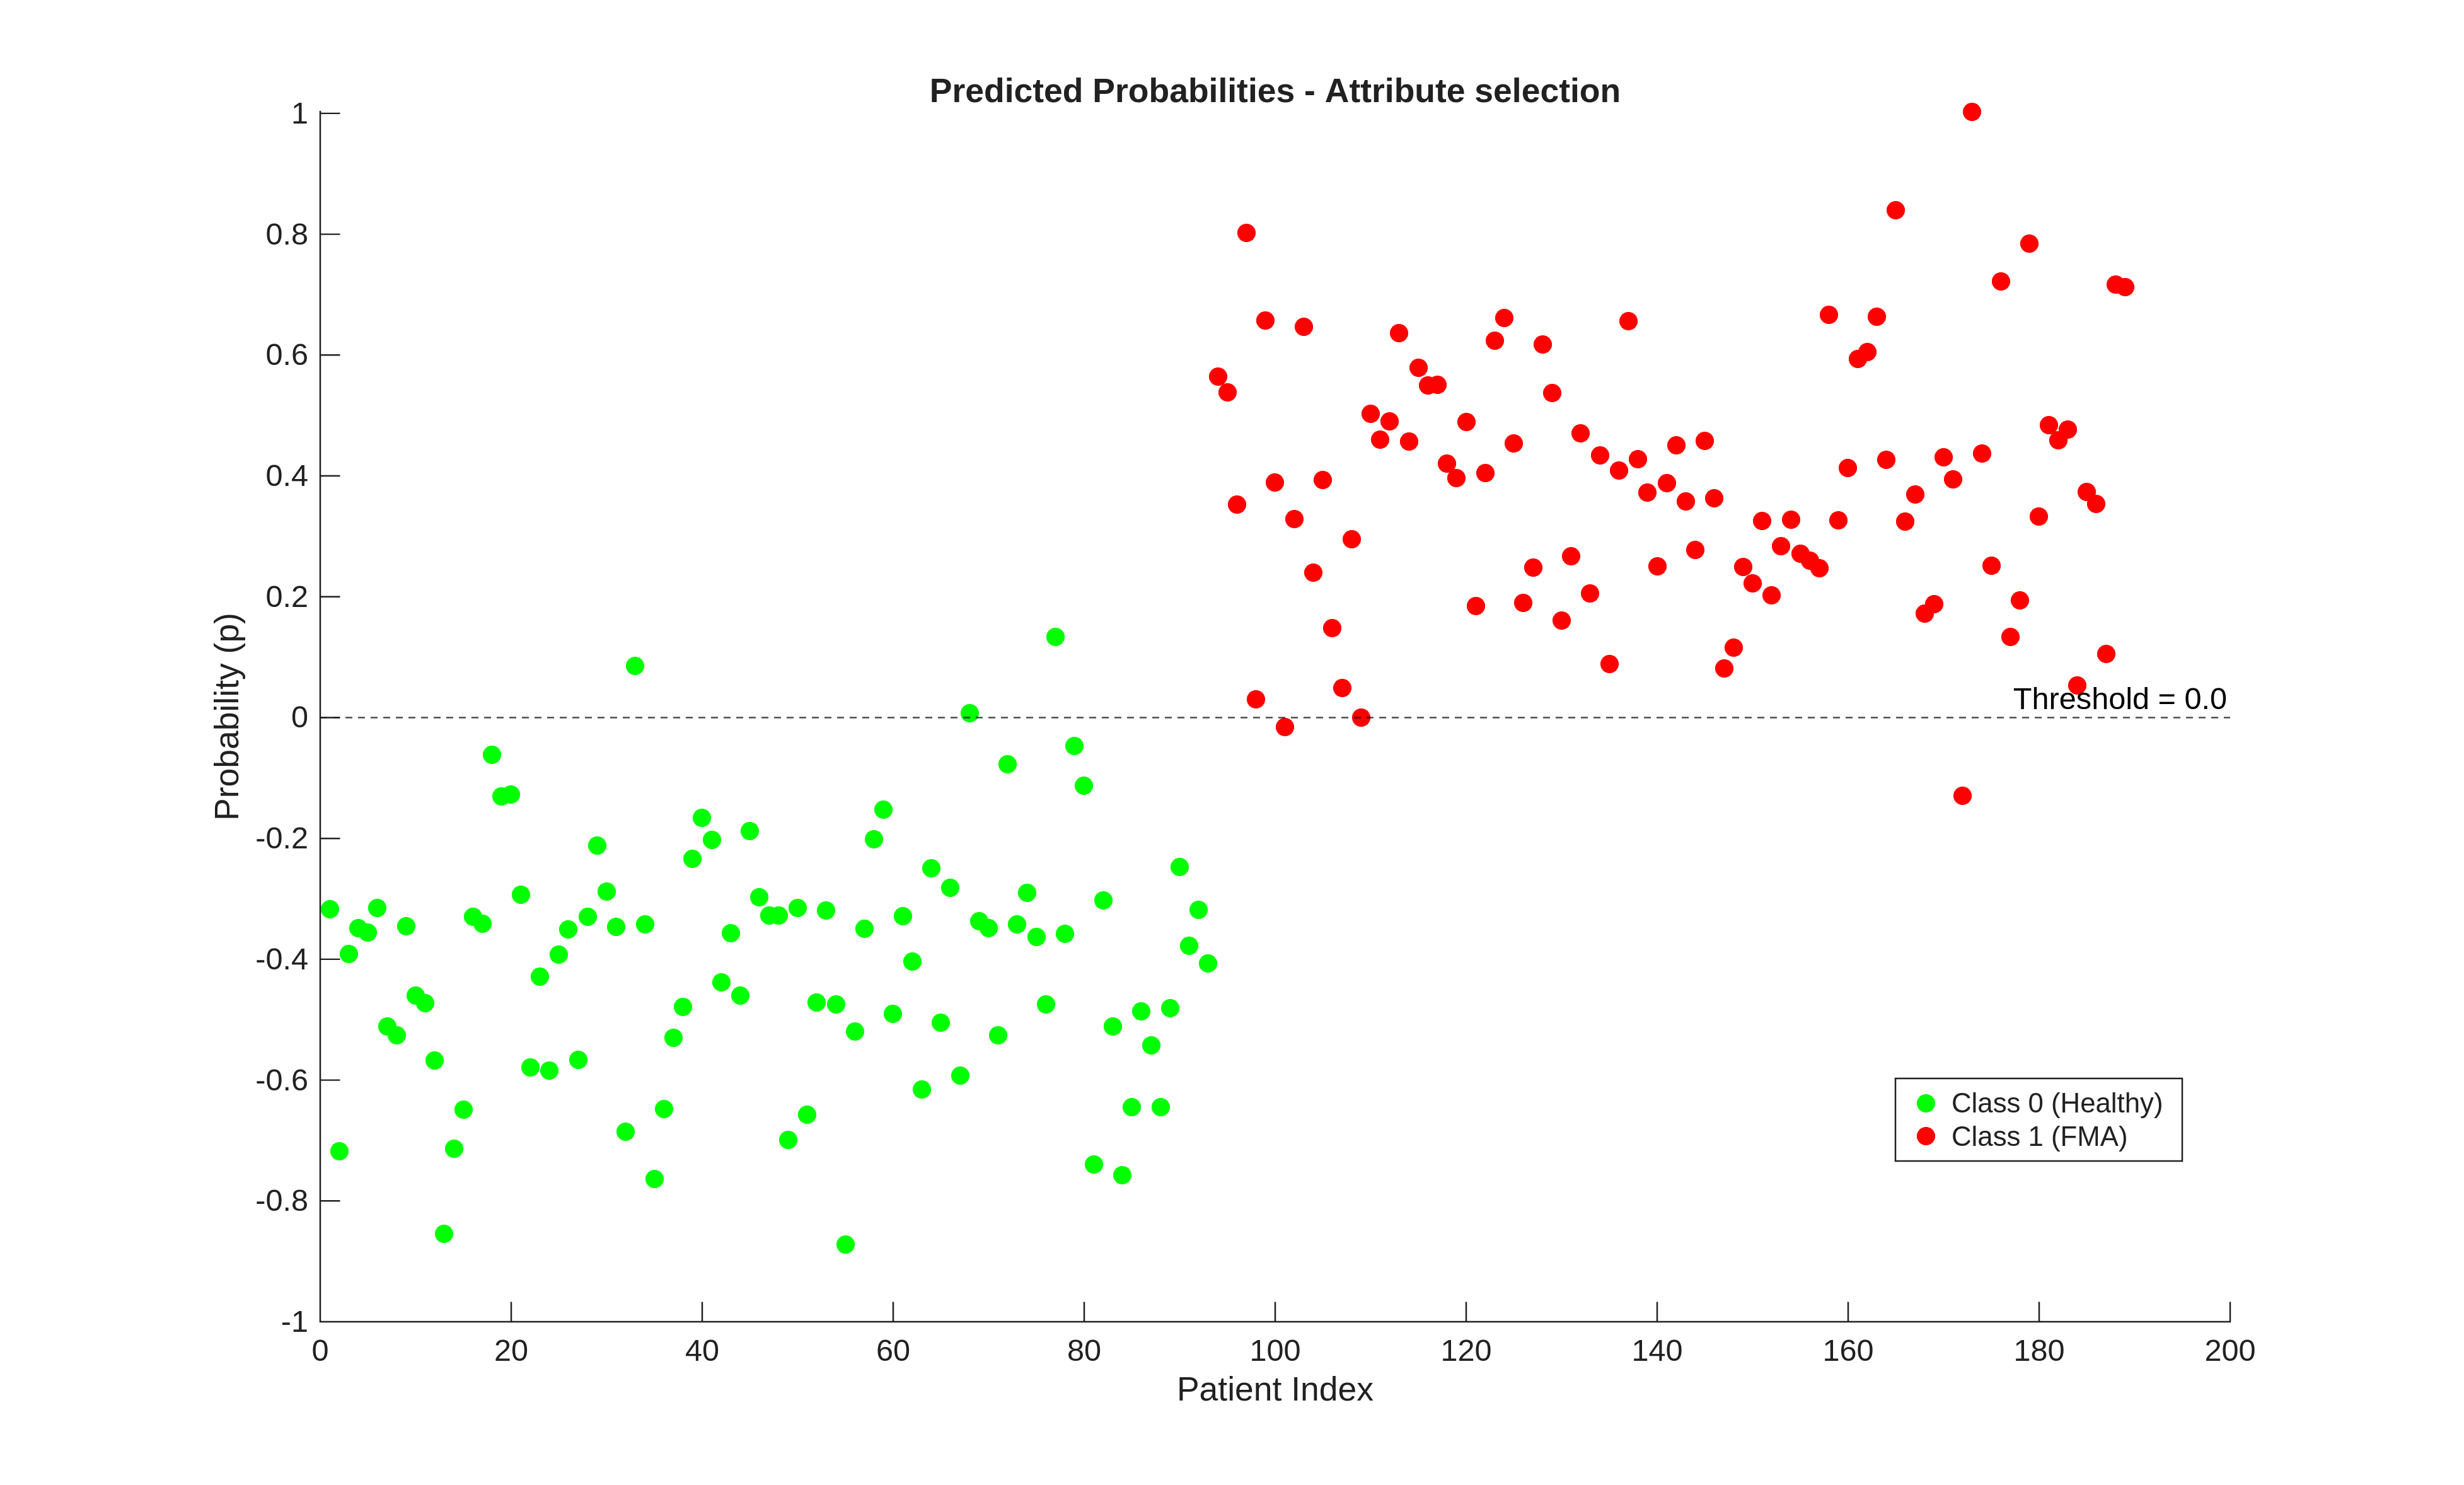
\includegraphics[width=\linewidth]{images/reduced_reg.png}
    \caption{Predicted probabilities ($p$) for patients using the optimal subset of attributes. Healthy controls (green) and FMA cases (red) show distinct separation around the $0.5$ threshold.}
    \label{fig:reg_log}
    \par\noindent\footnotesize\textit{Alt text: Scatter plot of predicted probability versus patient index for all 189 subjects; green points (healthy controls) cluster below a dashed horizontal threshold line at 0.5, while red points (FMA patients) cluster above it.}
\end{figure}

The automated chromosomal filtering outputted 33 target non-sexual genes, including \textit{PCSK5}, \textit{ASNS}, \textit{HAVCR1}, and \textit{BUB1}.

\subsection{SVD and Principal Components}
Analysis of the normalized singular values confirmed that the random and full matrices lacked clear hierarchical importance among dimensions due to overwhelming noise. Conversely, the reduced matrix $A_r$ displayed two to three dominating directions (Figure \ref{fig:svd_values}).

\begin{figure}[h]
    \centering
    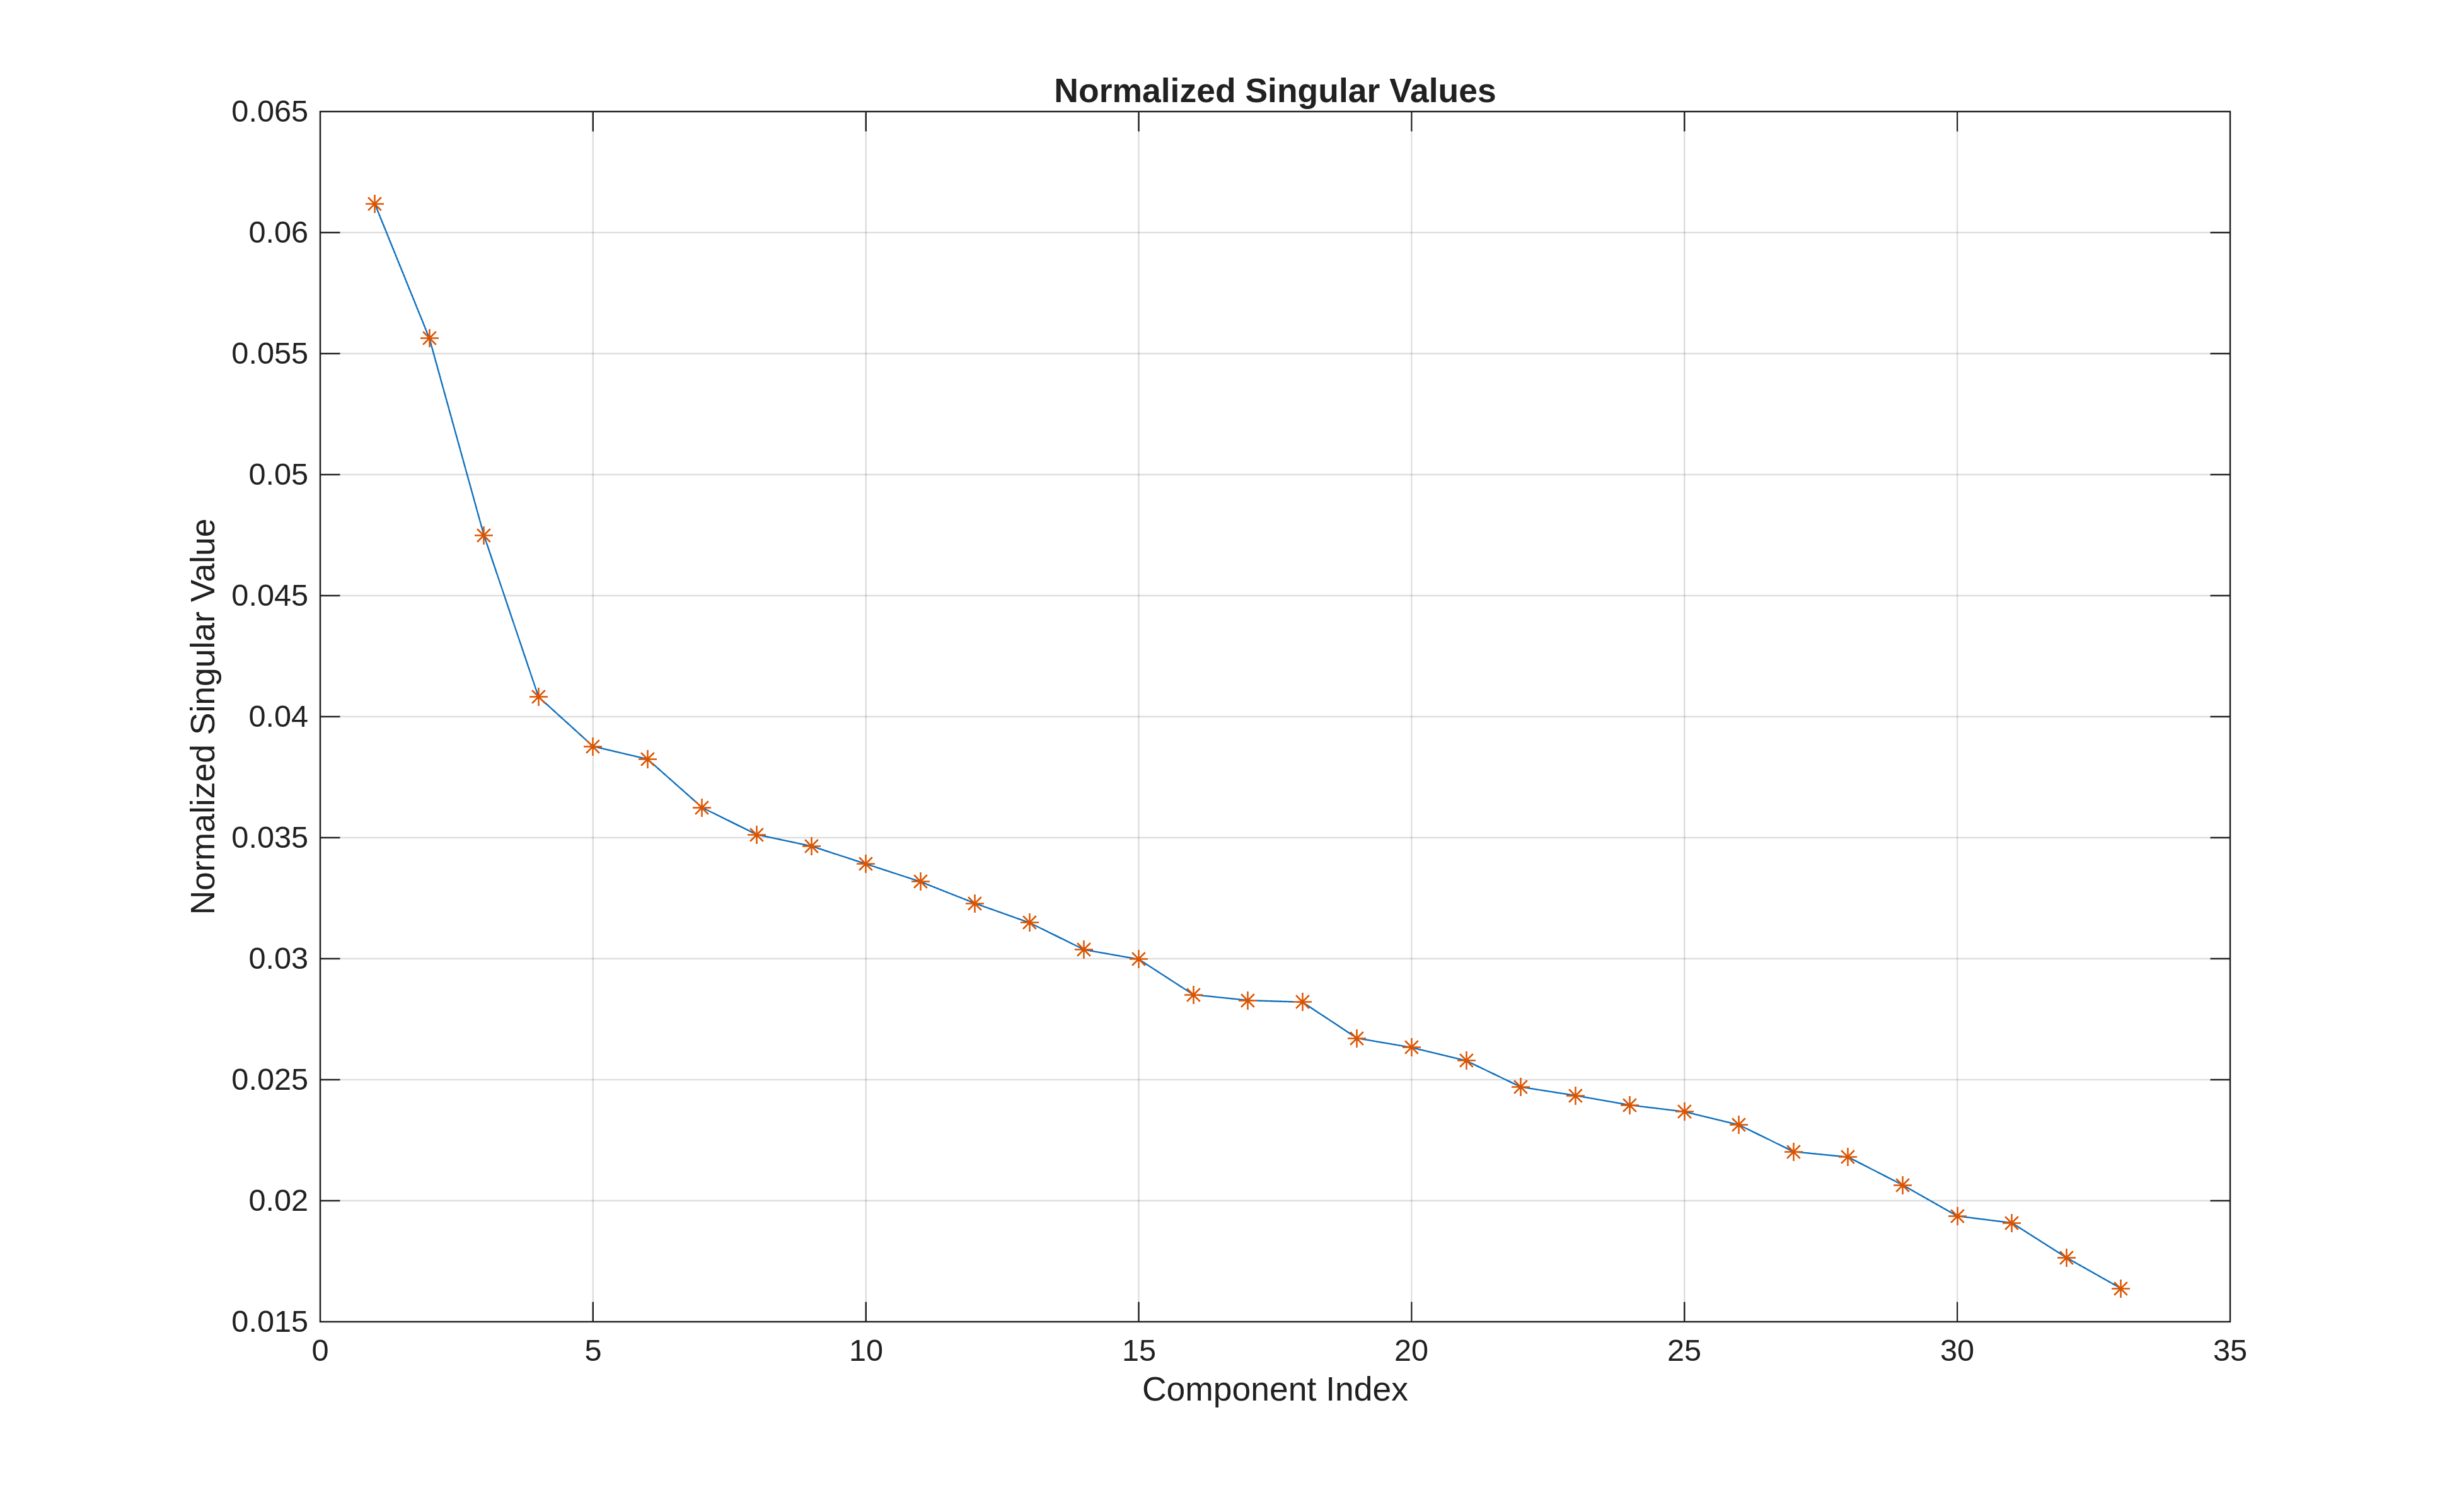
\includegraphics[width=\linewidth]{images/singular_values_reduced_2.png}
    \caption{Normalized singular values for the reduced 33-gene matrix. The sharp initial drop indicates a clear structural pattern overcoming the noise.}
    \label{fig:svd_values}
    \par\noindent\footnotesize\textit{Alt text: Line and scatter plot of normalized singular values (y-axis) against component index (x-axis), in descending order, showing two to three dominant values followed by a smooth, gradual decline for the remaining components.}
\end{figure}

By projecting the dataset onto the first three principal components, the 3D space plotting explicitly resolved the clusters of the two classes (Figure \ref{fig:svd_3d}), visually validating the feature selection's efficacy.

\begin{figure}[h]
    \centering
    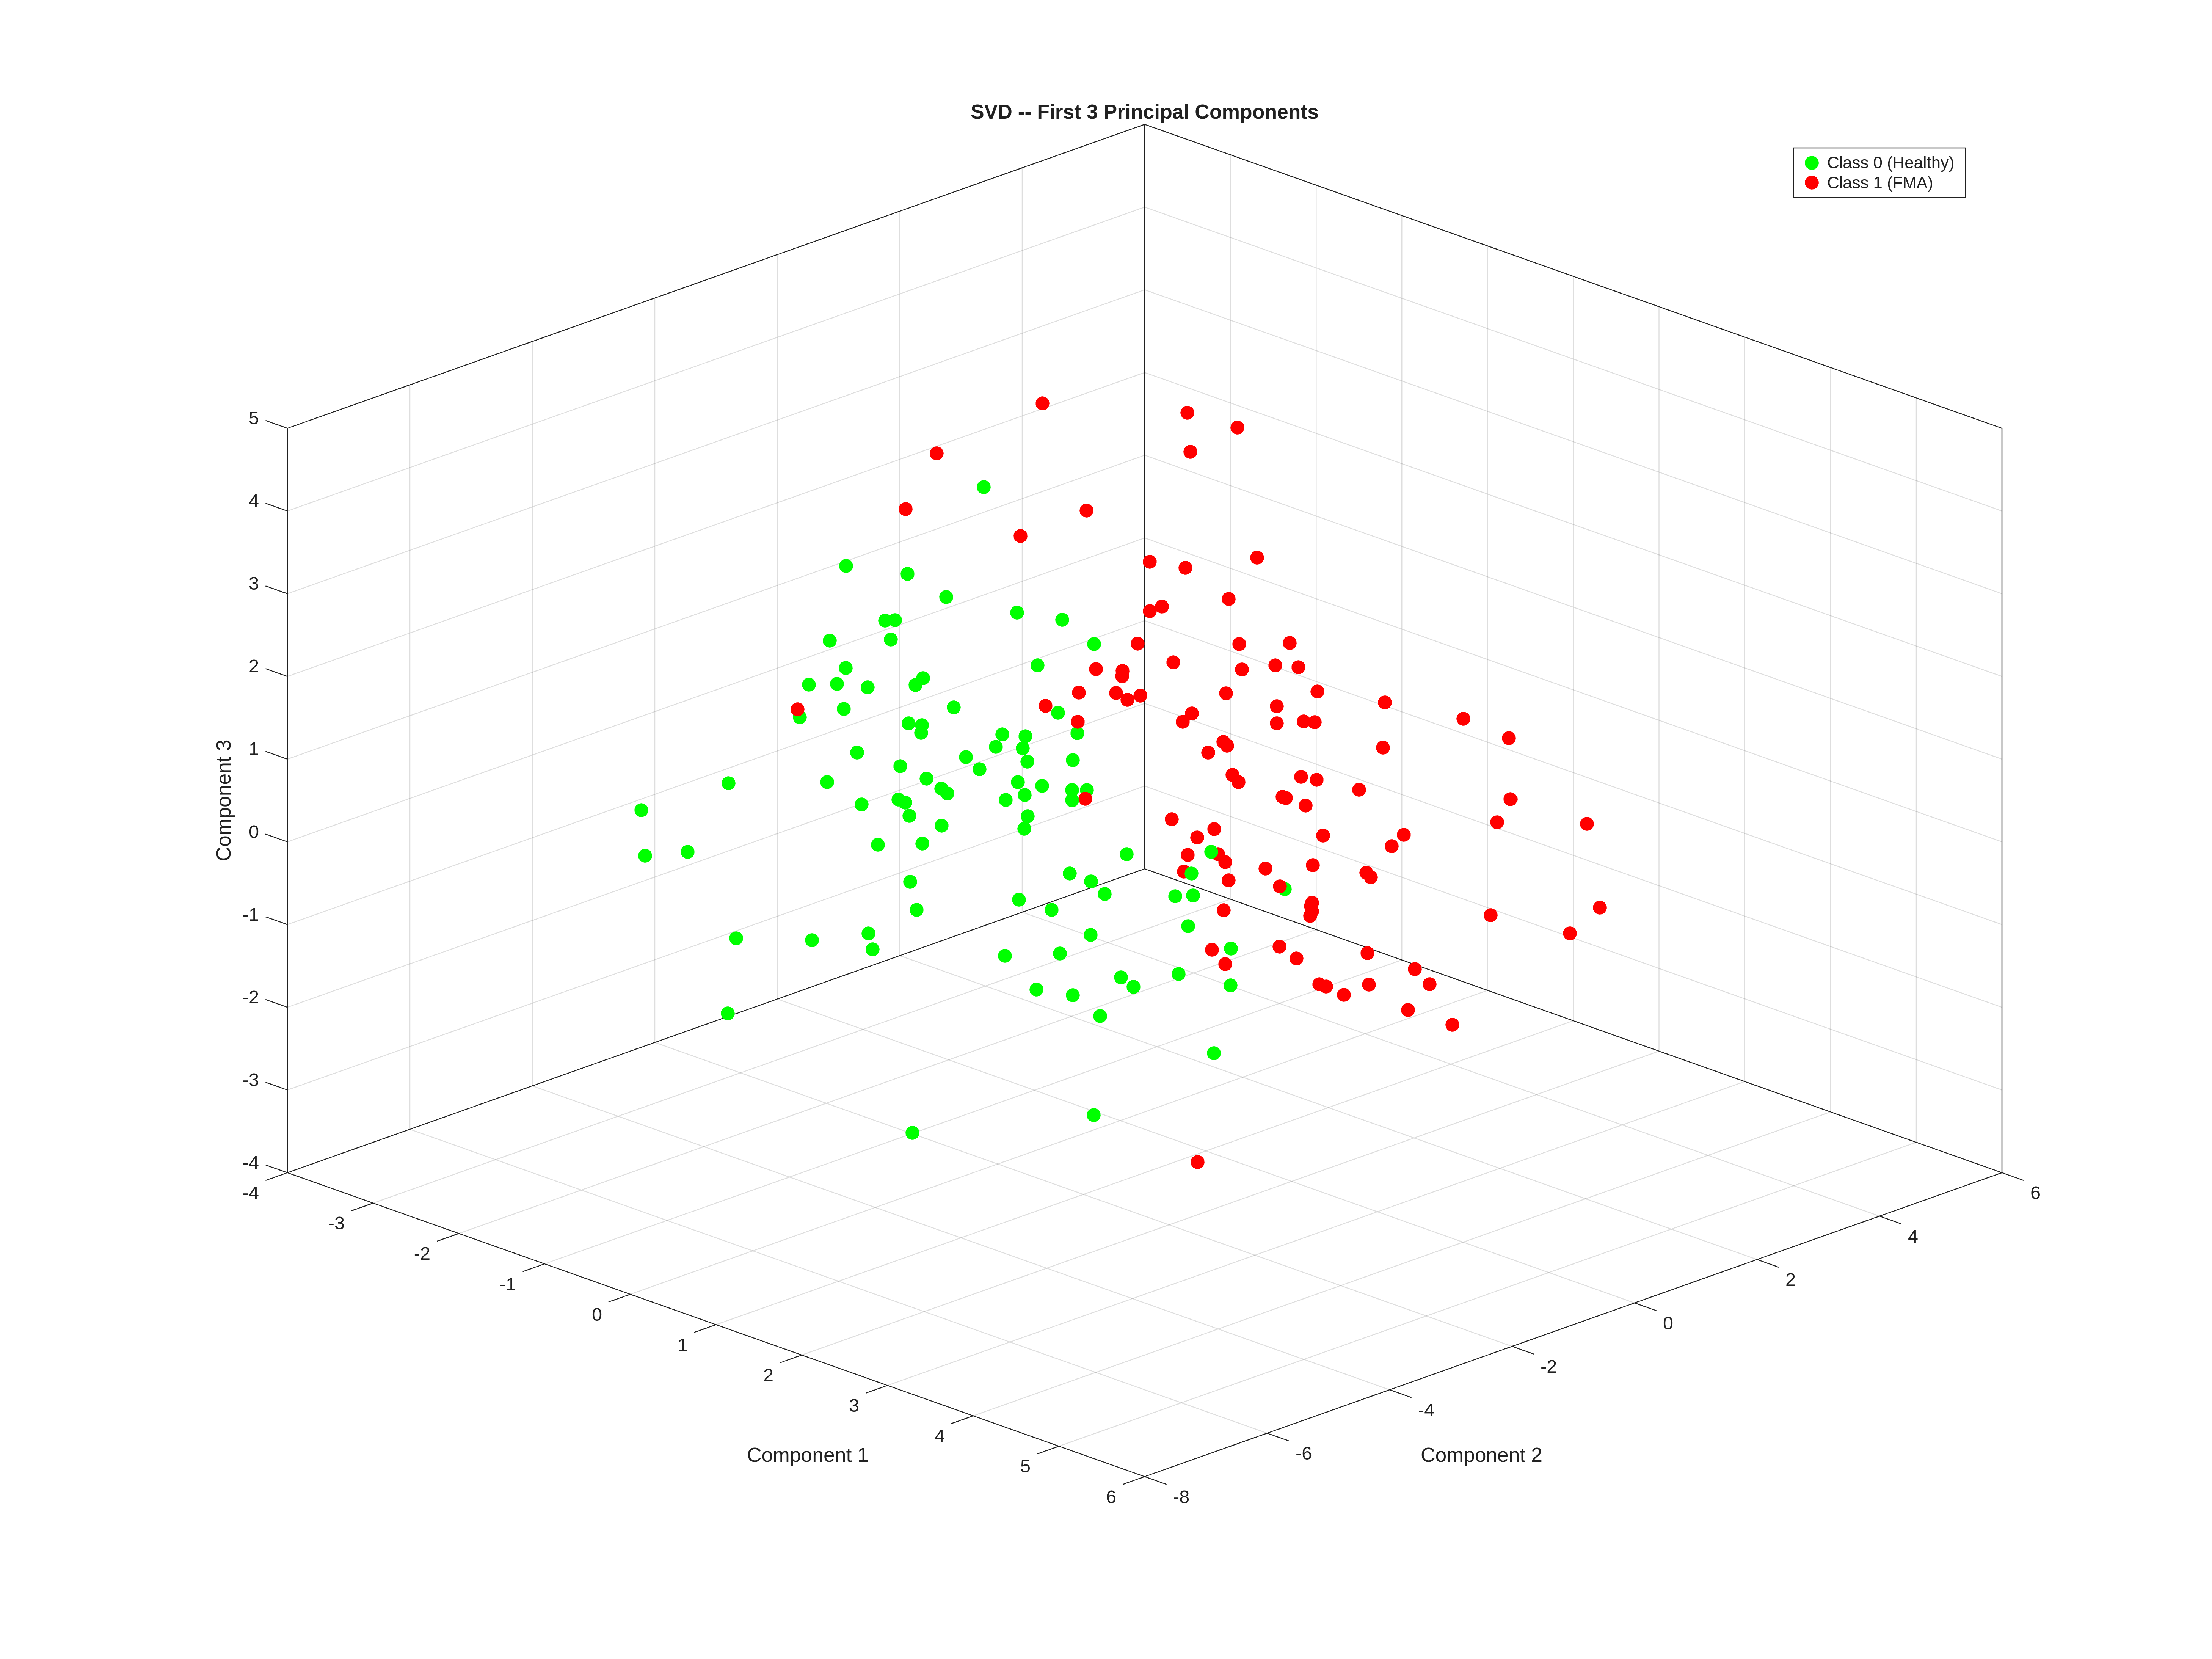
\includegraphics[width=\linewidth]{images/svd_results_reduced_2.png}
    \caption{3D Scatter plot of the first three principal components derived from SVD. The spatial distribution cleanly separates Class 0 (Healthy, green) from Class 1 (FMA, red).}
    \label{fig:svd_3d}
    \par\noindent\footnotesize\textit{Alt text: Three-dimensional gridded scatter plot with axes Component 1, Component 2, and Component 3, showing green points (healthy controls) and red points (FMA patients) forming two visually distinguishable spatial clusters.}
\end{figure}

\subsection{Classifier Performance}
The machine learning pipeline executing TruncatedSVD coupled with Logistic Regression was first evaluated on the independent holdout test set (30\% of the 189 samples, $n=57$), which was kept entirely unseen during the fitting of the scaler, the SVD components, and the classifier. Table~\ref{tab:holdout} reports the resulting accuracy, precision, recall, and F1-score for each class. By focusing strictly on the $n=5$ primary components, the estimator bypassed internal collinearity while retaining the discriminative structure observed in Figure~\ref{fig:svd_3d}.

\begin{table}[h]
    \centering
    \caption{Performance of the TruncatedSVD + Logistic Regression pipeline on the independent holdout test set ($n=57$ patients).}
    \label{tab:holdout}
    \begin{tabular}{lcccc}
        \toprule
        Class & Precision & Recall & F1-score & Support \\
        \midrule
        Healthy (0) & \texttt{0.93} & \texttt{1.00} & \texttt{0.97} & \texttt{28} \\
        FMA (1)     & \texttt{1.00} & \texttt{0.93} & \texttt{0.97} & \texttt{29} \\
        \midrule
        \multicolumn{4}{l}{Overall accuracy} & \texttt{96.49\%} \\
        \bottomrule
    \end{tabular}
\end{table}

As a complementary robustness check over the entire 189-sample dataset, the same pipeline was evaluated via Stratified 5-Fold Cross-Validation, achieving per-fold accuracies of 89.47\%, 86.84\%, 92.11\%, 97.37\%, and 94.59\%, with a mean accuracy of 92.08\% ($\pm$3.70\%), consistent with the holdout result above and confirming the predictive validity of the selected 33-gene cluster for FMA diagnostics.

% NOTE TO AUTHOR: replace the remaining placeholder values (\texttt{XX.XX}, \texttt{NN}, etc.) in Table~\ref{tab:holdout}
% with the actual numbers printed under "--- Resultados da Classificacao com SVD (Hold-out Test) ---" when running
% classifica_pacientes_svd.py. The 5-Fold CV sentence above has already been filled in.

\section{Discussion}
The primary obstacle in diagnosing Fibromyalgia is the noise-to-signal ratio in genomic transcriptions. Our findings show that relying on the full 21,446 gene matrix yields sub-optimal classifications obscured by biological noise. By performing a magnitude-based attribute selection and conservatively removing sex-linked genes, the SVD factorization proved that underlying patterns strongly differentiate healthy individuals from FMA patients. This methodology not only isolates reliable biological targets for future clinical assays but also provides a mathematically stable classification pipeline robust enough for small sample cohorts.

\textbf{Limitations.} While the final classification pipeline (Section 2.5) fits the scaler, the SVD components, and the logistic regression model exclusively on the training partition, the upstream attribute-selection and chromosomal-filtering steps (Sections 2.2--2.3) were performed on the complete 189-sample cohort prior to this split. Consequently, the 33 selected genes were chosen using information from samples that later compose the holdout test set, which may introduce a mild optimistic bias in the reported holdout and cross-validation accuracies. A more conservative evaluation would repeat attribute selection within each training fold (e.g.\ via nested cross-validation); we leave this refinement, together with external validation on an independent cohort, for future work.

\section*{Data Availability}
The RNA-Seq dataset analyzed in this study (GSE221921) is publicly available in the NCBI Gene Expression Omnibus (GEO) repository at \url{https://www.ncbi.nlm.nih.gov/geo/query/acc.cgi?acc=GSE221921}. All scripts used for data preprocessing, feature selection, chromosomal filtering, SVD, and classification (MATLAB and Python) are openly available at \url{https://github.com/GiorussoP/bioinformatics.git}.

\vspace{-1em}
\section*{Funding}
This work was supported by the Universidade Federal de Minas Gerais (UFMG).

\section*{Acknowledgements}
We thank the original authors of the GSE221921 dataset for making their RNA-Seq data publicly available via NCBI GEO. Generative AI tools (large language models) were used to assist in the drafting and revision of the manuscript text and in the generation of the MATLAB and Python code snippets used for data preprocessing, feature selection, and classification. All AI-assisted text and code were reviewed, validated, and edited by the author, who takes full responsibility for the accuracy and correctness of the final manuscript and implementation.

\begin{thebibliography}{9}
\bibitem{dataset}
[dataset] NCBI GEO, \textit{GSE221921: FM Processed Data}. Available at \url{https://www.ncbi.nlm.nih.gov/geo/query/acc.cgi?acc=GSE221921}.

\bibitem{hgnc}
HGNC Database, \textit{mygene.info} API. Accessed 2026.
\end{thebibliography}

\end{document}
